%Old Version from Greg. Greg, this slide is changed substantially, please take a look.
% begin module root-functions
%\begin{frame}
%\begin{itemize}
%\item<1->  If $n$ is a positive integer, the function $f(x) = x^{\frac{1}{n}} = \sqrt[n]{x}$ is called a root function.
%\item<2->  When $n = 2$, it is the square root function $f(x) = \sqrt{x}$.
%\item<3->  The square root is not defined for negative numbers, so its domain is $[0, \infty)$.
%\item<4->  Its graph is the top half of the parabola $x = y^2$.
%\item<5->  The graph of the cube root function $f(x) = \sqrt[3]{x}$ is similar to that of the square root, but it is defined everywhere.
%\end{itemize}
%\begin{tabular}{cc}
%\uncover<2->{%
%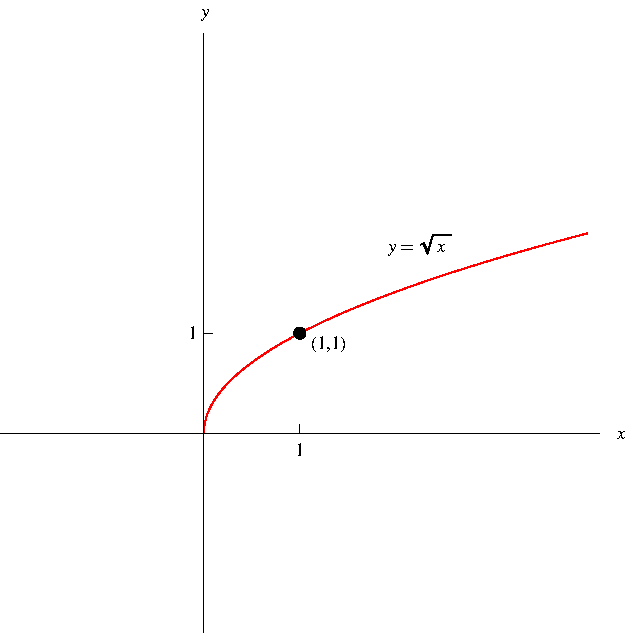
\includegraphics[height=3.5cm]{precalculus/pictures/01-02-sqrtx.pdf}%
%}%
%&%
%\uncover<5->{%
%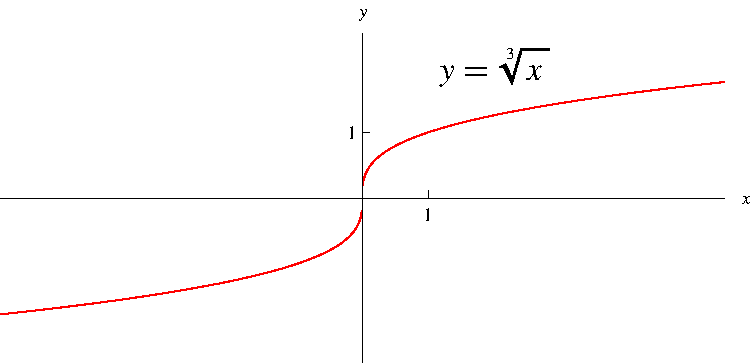
\includegraphics[height=3.5cm]{precalculus/pictures/cube-root.pdf}%
%}%
%\end{tabular}
%\end{frame}
% end module root-functions

% begin module root-functions
\begin{frame}
\begin{itemize}
\item<1->  $n$ - positive integer, $f(x) = x^{\frac{1}{n}} = \sqrt[n]{x}$ = the $n^{th}$ root function. $\sqrt[n]{x}\geq 0$ for $x\geq 0$. 
\item<2->  For $n = 2$, we get the square root $\sqrt{x}$; for $n=3$ we get the cube root $\sqrt[3]{x}$, and so on. 
\item<3-> Let $x>0$. For $n=2m+1$-odd, we can extend the definition of $n^{th}$ root to negative numbers by $ \sqrt[2m+1]{-x}:= -\sqrt[2m+1]{x}$. 
\item<4-> In this course, even roots of negative numbers are not defined.
\item<5-> The graph of $\sqrt{x}$ is the top half of the parabola $x = y^2$. \uncover<6->{Similarly for $y=\sqrt[2m]{x}$, we graph top of $x=y^{2m}$.}
\item<7->  The graph of the cube root $f(x) = \sqrt[3]{x}$ is the graph of the polynomial $x=y^3$. \uncover<8->{Similarly for $y=\sqrt[2m+1]{x}$, we graph $x=y^{2m+1}$}.
\end{itemize}
\begin{tabular}{cc}
\uncover<5->{%
\psset{xunit=0.6cm,yunit=0.6cm}
\tiny
\begin{pspicture}(-3,-2)(3.6,2)
\psaxes[labels=none]{<->}(0,0)(-3,-2)(3,2)
\rput[r](0,2){{$y$}}
\rput[l](3,0){{$x$}}
\uncover<handout:1|5>{
\psplot[linecolor=red]{0}{3}{ x 0.5 exp }
\rput( 3, 0.5){$y=\sqrt{x}$}
}
\uncover<handout:2|6->{
\psplot[linecolor=red, plotpoints=300]{0}{3}{ x 0.25 exp }
\rput( 3, 0.5){$y=\sqrt[4]{x}$}
}
\end{pspicture}
%\uncover<2->{%
%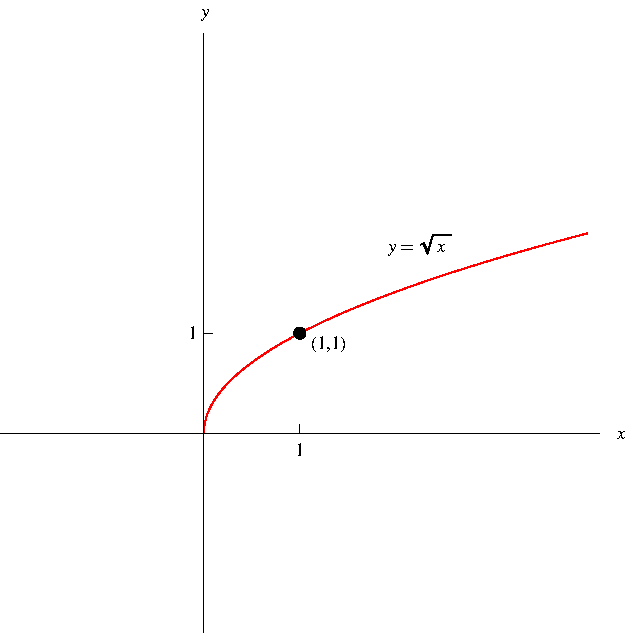
\includegraphics[height=3.5cm]{precalculus/pictures/01-02-sqrtx.pdf}%
%}%
}%
&%
\uncover<7->{%
\psset{xunit=0.6cm,yunit=0.6cm}
\tiny
\begin{pspicture}(-3,-2)(3.6,2)
\psaxes[labels=none]{<->}(0,0)(-3,-2)(3,2)
\rput[r](0,2){\tiny{$y$}}
\rput[l](3,0){\tiny{$x$}}
\uncover<handout:1|7>{
\psplot[linecolor=red, plotpoints=300]{-3}{0}{x -1 mul 0.3333 exp -1 mul}
\psplot[linecolor=red, plotpoints=300]{0}{3}{x 0.3333 exp }
\rput( 3, 0.5){$y=\sqrt[3]{x}$}
}
\uncover<handout:2|8->{
\psplot[linecolor=red]{-3}{0}{x -1 mul 0.2 exp -1 mul}
\psplot[linecolor=red]{0}{3}{x 0.2 exp }
\rput( 3, 0.5){$y=\sqrt[5]{x}$}
}
\end{pspicture}
}%
\uncover<handout:2|8->{}
\end{tabular}
\end{frame}
% end module root-functions